%%%
\chapter{Recursividade}

\section{Definições Recursivas de funções}

Em alguns casos, pode ser difícil definir um objeto explicitamente. Nestes casos, podemos definir um objeto em termos dele mesmo. Esse processo é chamado recursão.


Considere o seguinte exemplo: 

\begin{exemplo}
Uma linha de quadrados é construída usando palitos de fósforo, como mostrado na figura abaixo.


\begin{figure}[htbp]
\centering
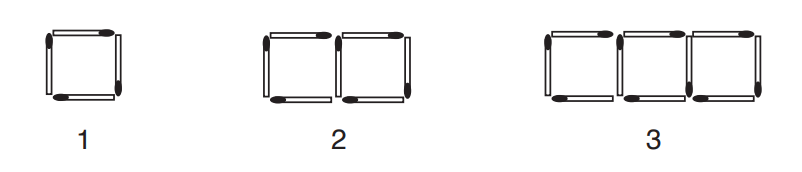
\includegraphics[width=.9\textwidth]{images/fosforos.png}
\label{fig:exampleFig2}
\end{figure}

Quantos palitos são necessários para a construção de uma linha de $n$ quadrados? 

Podemos definir uma função recursivamente para resolver este problema acima. A definição recursiva de uma função pode ser separada em dois casos:

\begin{itemize}
    \item Passo Base: Especifica o valor da função para o menor valor.
    \item Passo Recursivo: Apresenta uma regra para obter o valor para um número n a partir de casos menores.
\end{itemize}

Seja $f(n)$ o número de palitos necessários para construir uma linha de $n$ quadrados.

\begin{itemize}
    \item Passo Base: $f(1) = 4$
    \item Passo Recursivo: $f(n) = f(n-1) + 3$
\end{itemize}

Observe que juntando 3 novos palitos a linha de 1 quadrado podemos construir uma linha de 2 quadrados. No caso geral, se juntamos 3 novos palitos a uma linha de $n-1$ quadrados obtemos uma linha de $n$ quadrados.
\end{exemplo}

\newpage

\begin{exemplo}

João trabalha no supermercado, e seu gerente pediu que ele empilhasse latas de ervilhas como na figura abaixo.

\begin{center}
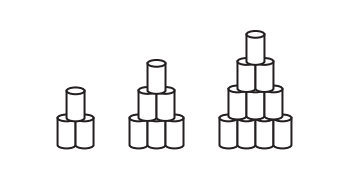
\includegraphics{images/Latas.png} 
\end{center}

Proponha uma definição recursiva para o número de latas necessárias para construir uma pilha de latas nesse formato com altura de $n$ latas. 

Seja $p(n)$ o número de latas necessárias para construir uma pilhas de latas no formato acima com uma altura $n$. Note que a pilha de altura 1 pode ser construída com apenas uma única lata.
Observe que podemos construir uma pilha de latas nesse formato com altura de $n$ latas, colocando $n$ latas na base e colocando a pilha de latas de altura $n-1$ sobre a base de $n$ latas. Dessa maneira, a definição recursiva para $p(n)$ será:

$$
p(n) = 
\begin{cases}
1 &  \text{ , $n$ =  1} \\
n + p(n-1) & \text{ , caso contrário}\\ 
\end{cases}
$$

\end{exemplo}





\begin{exemplo}
Imagine que você queira construir uma parede de tijolos com tijolos com o comprimento igual a duas vezes a sua altura. Considere que a nossa parede sempre terá apenas duas unidades de altura. Calcule de quantos padrões podemos construir uma parede com comprimento $n$.

\begin{figure}[!htbp]
\caption{Padrões de construções da parede com tijolos 1 x 2}
\label{fig::tijolos}
\begin{center}
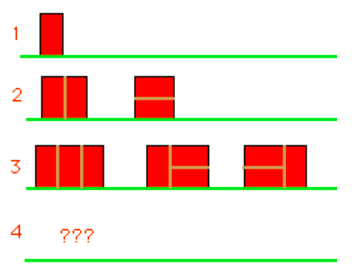
\includegraphics[scale=0.7]{images/pattern.png} 
\end{center}
\end{figure}

A Figura \ref{fig::tijolos} mostra a parede de comprimento igual a 3 pode ser construída de 3 maneiras diferentes.

Seja $t(n)$ o número de maneira de construir uma parede de comprimento $n$ com altura 2 usando apenas o tijolo 2x1. Note que podemos colocar o primeiro tijolo na parede de duas maneiras: um em pé ou dois tijolos deitados. Se colocarmos um tijolo em pé na parede de comprimento 3, podemos completar parede de duas maneiras diferentes ($t(2)$). Se o colocamos dois tijolos deitados, podemos completar a parede apenas de uma maneira ($t(1)$). O argumento acima está exemplificado na Figura \ref{fig::tijolos2}. De maneira geral,

$$t(n) = 
\begin{cases}
1 & n = 1\\
2 & n = 2\\
t(n-1) + t(n-2) & n \geq 3\\
\end{cases}
$$

\begin{figure}[!htbp]
\caption{Construção da parede usando o pensamento recursivo}
\label{fig::tijolos2}
\begin{center}
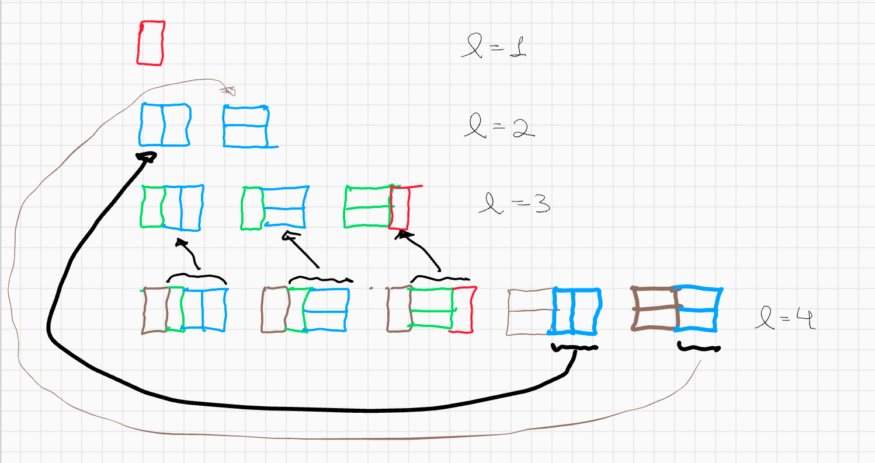
\includegraphics[scale=0.4]{images/tijolos.png} 
\end{center}
\end{figure}

\end{exemplo}



\begin{exemplo}
Você passa em uma loja perto de sua casa e vê a seguinte oferta: Uma garrafa de Choco Cola para cada 3 garrafas vazias devolvidas. Agora, você decide comprar algumas garrafas de cola nessa loja, quantas garrafas de cola você pode beber aproveitando essa promoção?

A Figura \ref{fig::chococola} mostra quantas garrafas de chococola você pode beber comprando inicialmente 8 garrafas de chococola.


\begin{figure}[!htbp]
\caption{Promoção chococola}
\label{fig::chococola}
\begin{center}
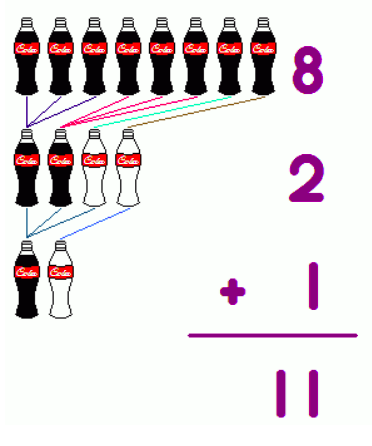
\includegraphics[scale=0.6]{images/cola.png} 
\end{center}
\end{figure}

Dê uma definição recursiva para a função $coca(n,m)$ que devolve o número de garrafas que você pode beber considerando que você tem $n$ garrafas cheias e $m$ garrafas vazias.



Primeiramente, vamos considerar os casos mais simples da função $coca(n,m)$:
$$coca(n,m) = 
\begin{cases}
0 & \text{, $m \leq 2 \wedge n = 0$}\\
n & \text{, $n \leq 2 \wedge m = 0$} 
\end{cases}
$$

Quando o número de garrafas vazias for menor ou igual a 2 e o número de garrafas cheias for zero não bebemos nenhuma garrafa. Quando o número de garrafas cheias for menor ou igual a 2 e o número de garrafas vazias for zero, bebemos apenas as garrafas cheias. 

Agora vamos considerar os casos mais complexos, vamos separar em dois casos:

$$coca(n,m) = 
\begin{cases}
coca(0, n+m) & \text{, $n \geq 0$}\\
coca(\lfloor m/3 \rfloor ,m \textbf{ mod } 3) & \text{, caso contrário} 
\end{cases}
$$

\end{exemplo}


\begin{exemplo}
3 objetos distintos podem ser organizados em sequência de seis maneiras diferentes.

\begin{center}
\begin{tabular}{c}
A,B,C\\
A,C,B\\
B,A,C\\
B,C,A\\
C,A,B\\
C,B,A\\
\end{tabular}
\end{center}

Dê uma definição recursiva para a função $f(n)$ que devolve o número de maneiras que podemos organizar n objetos distintos em sequência.

Seja f(n) o número de maneiras que podemos organizar n objetos distintos em uma sequência de tamanho $n$. O primeiro elemento de uma sequência pode ser escolhido de $n$ maneiras restando $n-1$ objetos para ser organizado em uma sequência de tamanho $n-1$. Logo,

$$
f(n) = 
\begin{cases}
1 & n = 1\\
n \cdot f(n-1) & \text{caso contrário}\\
\end{cases}
$$

\end{exemplo}

\begin{exemplo}



3 objetos distintos podem ser organizados em uma sequência de tamanho 2 de seis maneiras diferentes.

\begin{center}
\begin{tabular}{c}
A,B\\
A,C\\
B,A\\
B,C\\
C,A\\
C,B\\
\end{tabular}
\end{center}

Dê uma definição recursiva para a função $f(n, k)$ que devolve o número de maneiras que podemos organizar n objetos distintos em sequência de tamanho $k$ tal $k \leq n$.


Seja f(n,k) o número de maneiras que podemos organizar $n$ objetos distintos em uma sequência de tamanho $k$ tal que $k \leq n$. O primeiro elemento de uma sequência pode ser escolhido de $n$ maneiras restando $n-1$ objetos para ser organizado em uma sequência de tamanho $k-1$. Logo,

$$
f(n,k) = 
\begin{cases}
n & k = 1\\
n \cdot f(n-1,k-1) & \text{caso contrário}\\
\end{cases}
$$

\end{exemplo}

\begin{exemplo}{Números de triângulos em uma grade triangular}


\begin{minipage}{\textwidth}

Quantos triângulos em pé (tamanhos variados)
  podemos encontrar em uma grade de triângulos com
  altura $n$?
  
\begin{center}
    \begin{tikzpicture}
    \foreach \i in {0,1,2,3,4} {
      \draw (0 + 0.5*\i, \i * 0.5 * \sqrtofthree) -- (4 - 0.5*\i, \i * 0.5 * \sqrtofthree);
      \draw (0:\i) -- (60:\i);
      \draw[xshift=4cm] (180:\i) -- (120:\i);
    }
    \end{tikzpicture}
    \qquad
    \begin{tikzpicture}
    \fill[yellow!80] (0,0) -- (3,0) -- (1.5,3*0.5*\sqrtofthree);
    \fill[green!80] (1.5,0.5*\sqrtofthree) -- (3.5,0.5*\sqrtofthree) -- (2.5,3*0.5*\sqrtofthree);
    \foreach \i in {0,1,2,3,4} {
      \draw (0 + 0.5*\i, \i * 0.5 * \sqrtofthree) -- (4 - 0.5*\i, \i * 0.5 * \sqrtofthree);
      \draw (0:\i) -- (60:\i);
      \draw[xshift=4cm] (180:\i) -- (120:\i);
    }
    \end{tikzpicture}
  \end{center}

Destacamos dois triângulos de tamanhos variados encontrados em um triângulo de altura 4.

\end{minipage}


Seja $t(n)$ o número de triângulos em pé de tamanho variados que podemos encontrar em um grade triangulas com altura $n$.

Para uma grade de altura $n = 1$, temos $t(1) = 1$ triângulo

\begin{center}
    \begin{tikzpicture}
      \draw (0,0) -- (4,0) -- (2,4*0.5*\sqrtofthree) -- cycle;
    \end{tikzpicture}
  \end{center}
  
Para uma grade de altura $n = 2$, temos $t(2) = 4$ triângulo.

\begin{itemize}
  \item 2 com o vértice superior coincidindo com o vértice superior do maior triângulo.
  \item 2 outros triângulos com o vértice superior diferente do vértice superior do maior triângulo.
\end{itemize}

\begin{center}

\begin{tabular}{ll}

     \begin{tikzpicture}
      \foreach \i in {0,1,2} {
        \draw (0 + 1*\i, \i * 1 * \sqrtofthree) -- (4 - 1*\i, \i * 1 * \sqrtofthree);
        \draw (0:2*\i) -- (60:2*\i);
        \draw[xshift=4cm] (180:2*\i) -- (120:2*\i);
      }
      \draw[fill=blue!80] (1,\sqrtofthree) -- (3,\sqrtofthree) -- (2,2*\sqrtofthree) -- cycle;
      \draw[ultra thick, red!80] (0,0) -- (4,0) -- (2, 2*\sqrtofthree) -- cycle;
      \draw[ultra thick, red!80] (0,0) -- (4,0) -- (2, 2*\sqrtofthree) -- cycle;
    \end{tikzpicture}
&
         \begin{tikzpicture}
      \foreach \i in {0,1,2} {
        \draw (0 + 1*\i, \i * 1 * \sqrtofthree) -- (4 - 1*\i, \i * 1 * \sqrtofthree);
        \draw (0:2*\i) -- (60:2*\i);
        \draw[xshift=4cm] (180:2*\i) -- (120:2*\i);
      }
     
      \draw[fill=green!80] (0,0) -- (2,0) -- (1,\sqrtofthree) -- cycle;     
      \draw[fill=yellow!80] (2,0) -- (4,0) -- (3,\sqrtofthree) -- cycle;
      
    \end{tikzpicture}\\
\end{tabular}
  \end{center}

Podemos encontrar alguma padrão para $n=4$?

\begin{center}
    \begin{tikzpicture}
    
    
    
    
    \foreach \i in {0,1,2,3,4} {
      \draw (0 + 0.5*\i, \i * 0.5 * \sqrtofthree) -- (4 - 0.5*\i, \i * 0.5 * \sqrtofthree);
      \draw (0:\i) -- (60:\i);
      \draw[xshift=4cm] (180:\i) -- (120:\i);
    }
    \end{tikzpicture}
  \end{center}


Temos 4 triângulos têm o vértice superior coincidente com o vértice superior do triângulo maior

  \begin{center}
    \begin{tikzpicture}
      \fill[red!80]  (0,0) -- (4,0) -- (2, 2*\sqrtofthree) -- cycle;
      \fill[blue!80] (0.5,0.5 * \sqrtofthree) -- (3.5,0.5 * \sqrtofthree) -- (2, 4*0.5*\sqrtofthree) -- cycle;
      \fill[green!80] (1,\sqrtofthree) -- (3,\sqrtofthree) -- (2, 4*0.5*\sqrtofthree) -- cycle;
      \fill[yellow!80] (1.5,1.5*\sqrtofthree) -- (2.5,1.5*\sqrtofthree) -- (2, 4*0.5*\sqrtofthree) -- cycle;

      \foreach \i in {0,1,2,3,4} {
        \draw (0 + 0.5*\i, \i * 0.5 * \sqrtofthree) -- (4 - 0.5*\i, \i * 0.5 * \sqrtofthree);
      }
      \draw (0,0) -- (4,0) -- (2,4*0.5*\sqrtofthree) -- cycle;
    \end{tikzpicture}
  \end{center}
  
Os outros triângulos cujos vértices superiores não coincidem com o vértice superior do triângulo maior podem aparecer nesses dois triângulos amarelos internos (t(n-1)). Observe que somamos todos os triângulos que estão nos dois triângulos amarelos, os triângulos que estão dentro do triângulo vermelho (t(n-2)) serão contados duas vezes




\begin{center}
        \begin{tikzpicture}
          \foreach \i in {0,1,2,3,4} {
            \draw (0 + 0.5*\i, \i * 0.5 * \sqrtofthree) -- (4 - 0.5*\i, \i * 0.5 * \sqrtofthree);
            \draw (0:\i) -- (60:\i);
            \draw[xshift=4cm] (180:\i) -- (120:\i);
          }
          \draw[fill=yellow!80] (1,0) -- (4,0) -- (2.5, 3*0.5*\sqrtofthree) -- cycle;
          \draw[fill=yellow!80] (0,0) -- (3,0) -- (1.5, 3*0.5*\sqrtofthree) -- cycle;
          \draw[fill=red]  (1,0) -- (3,0) -- (2,   2*0.5*\sqrtofthree) -- cycle;
        \end{tikzpicture}
\end{center}

A definição recursiva de $t(n)$ é:
$$
t(n) =
\begin{cases}
1  & n = 1 \\
4  & n = 2 \\
n + 2 \cdot t(n-1) - t(n-2) & n \geq 3\\
\end{cases}
$$

\end{exemplo}


\begin{exemplo}

Ao subir a escada de seu prédio, José às vezes sobe dois degraus de uma vez e às vezes sobe um de cada
vez. Sabendo que a escada tem 3 degraus, de quantas maneiras diferentes José pode subir a escada? Você
consegue generalizar para o caso de uma escada com $n$ degraus?


Primeiramente, vamos pensar nos casos menores:

\begin{itemize}
    \item Uma escada de 1 degrau, podemos subir as escadas de 1 maneira (1).
    \item Uma escada de 2 degrau, podemos subir as escadas de 2 maneiras (1+1,2).
    \item Uma escada de 3 degraus, podemos subir as escadas de 3 maneiras (1+1+1,1+2,2+1).
\end{itemize}

Seja $x_n$ número de maneira de subir uma escada de $n$ degraus.  O primeiro passo para subir uma escada de n degraus pode ser dado de duas maneiras:

\begin{itemize}
    \item Se você subir apenas um degrau, então teremos $x_{n-1}$ maneiras de subir o restante da escada.
    \item Se você subir dois degraus, então teremos $x_{n-2}$ maneiras de subir o restante da escada.
\end{itemize}

A recorrência para $x_n$ será:

$$
x_n = \begin{cases}
1 & n = 1\\
2 & n = 2\\ 
x_{n-1} + x_{n-2} & n \geq 3\\
\end{cases}
$$
\end{exemplo}

\begin{exemplo}
Quantas são as sequências de n termos pertencentes a \{0,1\} , que possuem um número ímpar de termos iguais a 0?

Por exemplo,

Sequências de tamanho 1: 1 (0) 

Sequências de tamanho 2: 2 ( 01 e 10)

Encontre uma relação de recorrência que relaciona o número de termos dessa sequência.

Seja f(n) o número de sequências de $n$ termos 0 e 1 com uma quantidade ímpar de termos iguais a 0. O número de sequência de $n+1$ termos 0 e 1 com um número ímpar de termos iguais a 0 é igual a soma:
\begin{itemize}
    \item do número de sequências começadas por 1 seguido por uma sequência de $n$ termos com um número ímpar de zeros 
    \item com o número de sequências começadas por zero seguido por um sequência de $n$ termos com um número par de zeros.
\end{itemize}


Portanto,

\begin{equation}
    f(n+1) = f(n) + 2^n - f(n) = 2^n
\end{equation}

Logo,

\begin{equation}
    f(n)  = 2^{n-1}
\end{equation}

\end{exemplo}

\section{Exercícios}


\begin{enumerate}
\item 



Suponha que um par de coelhos recém-nascidos, um macho e uma fêmea, sejam colocados em um campo. Os coelhos podem acasalar com um mês de idade, de modo que no final do segundo mês uma fêmea pode produzir outro casal de coelhos. Suponha que nossos coelhos nunca morram e que a fêmea sempre produz um novo par (um macho, uma fêmea) a cada mês a partir do segundo mês.  

\begin{center}
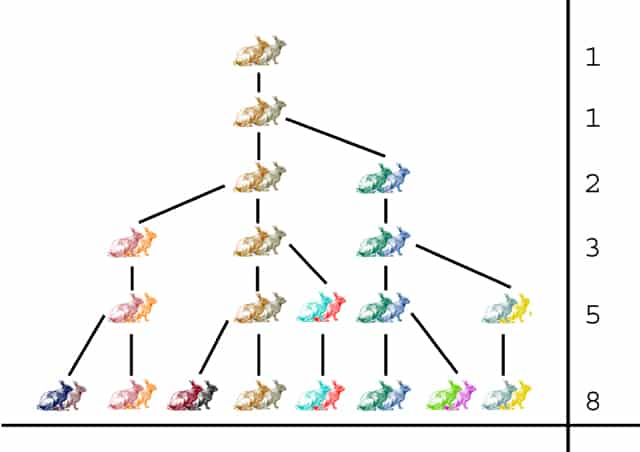
\includegraphics[scale=0.4]{images/rabbits.jpg} 
\end{center}

A imagem mostra que ao final do sexto mês teremos 8 pares de coelhos.


Quantos pares de coelhos teremos ao final de n meses?

Desenvolva uma função recursiva $f(n)$ que devolve o número de pares de coelhos após $n$ meses.

\item 




Suponha agora os nossos coelhos não vivam para sempre e morrem depois de k meses. Contudo, os coelhos acasalam com um mês de idade e cada fêmea produz um novo par de coelhos a cada mês a partir do segundo mês.


\begin{center}
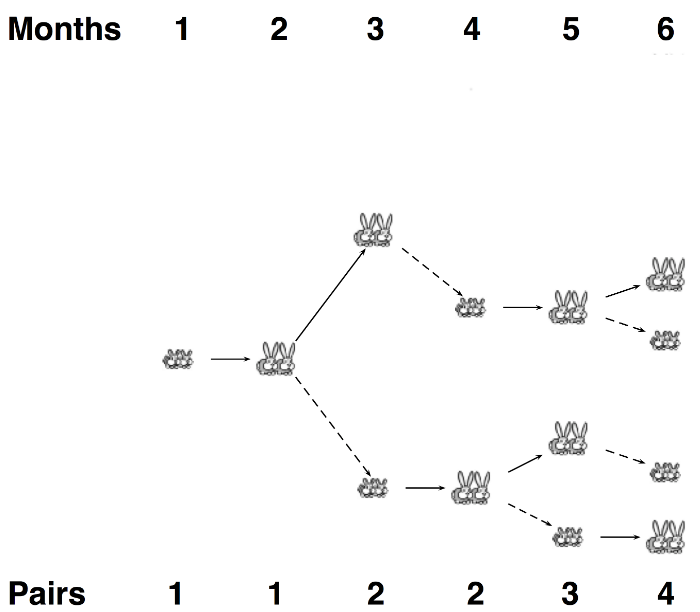
\includegraphics[scale=0.4]{images/rabbits2.png} 
\end{center}

A imagem mostra que ao final de seis meses teremos apenas 4 pares de coelhos considerando que os coelhos morrem após 3 meses.

Quantos pares de coelhos teremos ao final de n meses?

Desenvolva uma função recursiva $f(n,k)$ que devolve o número de pares de coelhos após $n$ meses considerando que os coelhos morrem depois de k meses. 



\item 

Ao subir a escada de seu prédio, José  sobe 1, 2 ou 3 degraus de uma vez. Sabendo que a escada tem 5 degraus, de quantas maneiras diferentes José pode subir a escada? Você
consegue generalizar para o caso de uma escada com $n$ degraus?

\item 

Quantas são as sequências de n termos pertencentes a \{0,1,2\} , que não possuem dois zeros consecutivos?

Por exemplo,

Sequências de tamanho 1: 3 (0,1 e 2) 

Sequências de tamanho 2: 8 ( 01,02,10,11,12,20,21 e 22)

\item 

Quantas são as sequências de n termos pertencentes a \{0,1,2\} , que não possuem dois zeros consecutivos?

Por exemplo,

Sequências de tamanho 1: 3 (0,1 e 2) 

Sequências de tamanho 2: 8 ( 01,02,10,11,12,20,21 e 22)

Faça um programa que gere todas as sequências de tamanho $n$ com termos pertencentes  a \{0,1,2\} , que não possuem dois zeros consecutivos.


\item 

Quantas são as sequências de n termos pertencentes a \{0,1,2\} , que possuem um número ímpar de termos iguais a 0?

Por exemplo,

Sequências de tamanho 1: 1 (0) 

Sequências de tamanho 2: 4 ( 01, 10, 20 e 02)

Encontre uma relação de recorrência que relaciona o número de termos dessa sequência.

\item 

Renata montou uma sequência de triângulos com palitos de fósforo, seguindo o padrão indicado na figura abaixo.

\begin{center}
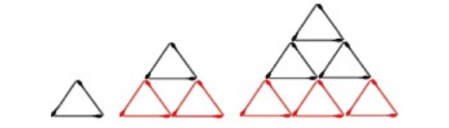
\includegraphics[width=1.0\linewidth,scale=0.8]{images/palitos.png} 
\end{center}

Quantos palitos serão usados por Renata no n-ésimo termo dessa sequência?

\item
Começando com um quadrado de 1cm de lado, formamos uma sequência de figuras, ob-
serve a figura abaixo. Cada figura, a partir da segunda, é formada unindo-se três cópias
da anterior. Os contornos destacados em vermelho das quatro primeiras figuras medem,
respectivamente, 4cm, 8cm, 20cm e 56cm. Quanto mede o contorno da figura n?


\begin{center}
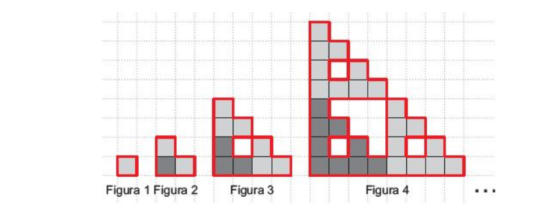
\includegraphics[width=1.0\linewidth,scale=0.8]{images/figura_recursiva.png} 
\end{center}

\item 

Um convidado em uma festa é uma celebridade se essa pessoa for conhecida por todos os outros convidados, mas não conhece nenhum deles. Existe no máximo uma celebridade em uma festa, pois se houvesse duas, eles se conheceriam.. Uma festa particular pode não ter celebridade. Sua tarefa é encontrar a celebridade, se ela
existe, em uma festa, fazendo apenas um tipo de pergunta - perguntando a um convidado se ele conhece um segundo convidado. Todos devem responder às suas perguntas com sinceridade. Ou seja, se Alice e Bob são duas pessoas na festa, você pode perguntar a Alice se ela conhece Bob; ela deve responder corretamente.

Seja $G(n)$ o número de perguntas utilizada para encontrar uma celebridade em uma festa com n pessoas.

\begin{enumerate}
    \item Calcule $G(1)$, $G(2)$, $G(3)$
    \item Proponha uma definição recursiva para $G(n)$. [Dica: primeiro faça uma pergunta para eliminar uma pessoa como celebridade. Em seguida, identifique  uma celebridade em potencial. Por fim, faça mais duas perguntas para determinar se a celebridade em potencial é na verdade uma celebridade.]
\end{enumerate}


\item 

Suponha que existem $n$ pessoas em um grupo, cada pessoa está ciente de um escândalo que
ninguém mais no grupo sabe sobre. Essas pessoas conversam por telefone; quando duas pessoas no grupo conversam, elas compartilham informações sobre todos os escândalos que cada um conhece. Para
por exemplo, na primeira chamada, duas pessoas compartilham informações, então
ao final da ligação, cada uma dessas pessoas sabe sobre dois escândalos. O problema da fofoca pede $G(n)$, o mínimo número de chamadas telefônicas necessárias para todas as n pessoas para
aprenda sobre todos os escândalos. 

\begin{enumerate}
    \item Mostre $G(1) = 0$
    \item Mostre $G(2) = 1$
    \item Mostre $G(3) = 3$
    \item Mostre $G(4) = 4$
    \item Mostre $G(5) = 6$
    \item Proponha um definição recursiva para $G(n)$
    
    
\end{enumerate}

\end{enumerate}













\section{Algoritmo Recursivo}

Um algoritmo é dito recursivo quando ele resolve um problema reduzindo para uma instância do mesmo problema com uma entrada menor.

\begin{exemplo}{Exponenciação}

Considere a seguinte definição recursiva da exponenciação:

\begin{equation}
a^n = 
\begin{cases}
1           & , n = 0\\
a * a^{n-1} & , n \geq 1
\end{cases}
\end{equation}
\end{exemplo}
O algoritmo recursivo para calcular $a^n$:

\begin{minted}{C++}
int exp(int a, int n){
	if(n==0) return 1;
	else return a*exp(a, n-1);
}
\end{minted}



No algoritmo acima, realizamos $n-1$ multiplicações para calcular $a^n$. Podemos fazer melhor utilizando uma outra definição recursiva.


\begin{exemplo}{Exponenciação rápida}

\begin{equation}
a^n = 
\begin{cases}
1           & , n = 0\\
(a^{n/2})^2 & , \text{$n$ é par}\\
a * a^{n-1} & , \text{$n$ é ímpar}

\end{cases}
\end{equation}
\end{exemplo}
\begin{minted}{C++}
int fast_exp(int a, int n){
    if(n==0) return 1;
    if(n%2==0){
        int res = fast_exp(a,n/2);
        return res*res;
    }else{
        return a*fast_exp(a, n-1);
    }
    
}
\end{minted}




\begin{exemplo}{soma de um vetor}

A definição recursiva da soma dos elementos de um vetor $a$ com índices variando entre $start$ e $end$:

\begin{equation}
soma(a, start, end) = 
\begin{cases}
a[start]           & , start = end\\
a[start] + soma(a, start+1, end) & , \text{caso contrário}\\

\end{cases}
\end{equation}


O algoritmo recursivo para calcular a soma dos elementos entre os duas posições start e end.

\begin{minted}{C++}
int soma_vetor(int *a, int start, int end){
	if( start == end ){
		return a[start];
	}else{
		return a[start] + soma_vetor(a, start + 1, end);
	}
}
\end{minted}

\end{exemplo}

\begin{exemplo}{Palavra palíndroma}

Considere a definição recursiva da função $is\_palindrome(s,i,j)$  que verificar se um palavra $s[i\ldots j]$ é palíndroma :

\begin{equation}
is\_palindrome(a, start, end) = 
\begin{cases}
true , start > end\\
true , start = end\\
s[start] == s[end] \&\& is\_palindrome(s, start+1, end-1)  \text{, caso contrário}\\

\end{cases}
\end{equation}




Observe que para testar se uma palavra com tamanho maior ou igual a 2, precisamos testar se o primeiro e o último caractere são iguais, depois precisamos testar se a palavra obtida pela remoção do primeiro e do último caractere  também é palíndroma.

\begin{minted}{C++}
bool is_palindrome(char s[], int i, int j){
    
    //palavra vazia
    if( i  > j ) return true;  
    //palavra de tamanho 1
    if( i == j ) return true; 
    
    if( s[i] == s[j] )
        return is_palindrome(s, i+1, j-1);
    else
        return false;
    
}
\end{minted}

\end{exemplo}


\begin{exemplo}{Busca linear}

Dado um vetor não-ordenado de inteiros de tamanho $n$ ( $a_0,a_1, \ldots, a_{n-1}$) e um um inteiro x. Implemente a função $busca(a, i, j, x)$ que devolve o índice da primeira ocorrência de x no subvetor $a_i, a_{i+1}, \ldots, a_j$, caso contrário, devolve -1. 

A função $busca(a, i, j, x)$ pode ser definida recursivamente da seguinte maneira:

\begin{equation}
busca(a, i, j , x) = 
\begin{cases}
  i, \text{se } A[i] = x\\
 -1, \text{se } i == j \\
busca(a, i+1, j, x) \text{, caso contrário}\\

\end{cases}
\end{equation}

\begin{minted}{C++}
int busca( int * A, int i, int j, int x){
    if( A[i] == x ) return i;
    else if(i == j) return -1;
    else return busca(A, i+1, j, x);
}
\end{minted}


\end{exemplo}

\begin{exemplo}
Dado um vetor de inteiros $arr$ de tamanho n existe uma posição k tal que 

$$arr[0] < arr[1] < ... < arr[k] > arr[k+1] > arr[k+2] > ... > arr[n-1]$$

Descubra $k$ usando a busca binária.

A função $pico(a, p, r)$ que devolve o valor de $k$ no intervalo $[p,r]$ pode ser definida recursivamente

\begin{equation}
pico(A, p, r) = 
\begin{cases}
  p  & \text{, se } p = r\\
  max(A[p],A[r]) & \text{, se } r == p+1 \\
  mid & \text{,} A[mid] > A[mid-1] \text{ e } A[mid] > A[mid+1]  \\
  pico(A, mid+1,r)      & \text{,} A[mid] < A[mid+1] \text{ e } A[mid-1] < A[mid]   \\
  pico(A, p,mid-1)      & \text{,} A[mid-1] > A[mid]    \\
\end{cases}
\nonumber 
\end{equation}
onde mid = (p+r)/2;


\begin{minted}{C++}
int pico(vector <int> & A, int p, int r){
    if( r-p == 0 ){ // tamanho 1
        return p;
    }else if( r-p == 1){ // tamanho 2 
        if(A[p] > A[r]) return p;
        else return r;
    }else{ // tamanho 3 ou mais
        int mid = p+r/2;
        if(A[mid] > A[mid-1] && A[mid] > A[mid+1]) return mid;
        if( A[mid-1] < A[mid]){
            if( A[mid] > A[mid+1] ) return mid;
            else{ // A[mid] < A[mid+1]
                return pico(A, mid+1, r);
            }
        }else{ // A[mid-1] > A[mid]  
            return pico(A, p, mid-1);
        }    
    }
}

\end{minted}
    
\end{exemplo}



\section{Exercícios}

\begin{enumerate}
    \item Proponha um algoritmo recursivo para encontrar o máximo de um vetor de tamanho $n$ usando o fato que o máximo de n inteiros é o maior entre o último inteiro do vetor e o máximo dos primeiros n-1 inteiros do vetor. 
    
    \item Proponha um algoritmo recursivo para computar o maior divisor comum de dois inteiros não negativos $a$ e $b$ com a  < b usando o fato que $mdc(a,b) = mdc(a, b-a)$. Note que se um número $d$ divide $a$ e $b$ então ele divide $a$ e $b-a$.
    
    \item Proponha um algoritmo recursivo para encontrar a primeira ocorrência de um valor x em um vetor ordenado de tamanho $n$ ( $a_0,a_1, \ldots, a_{n-1}$). Implemente a função $busca(a, i, j, x)$ que procura a primeira ocorrência de x no subvetor $a_i, a_{i+1}, \ldots, a_j$. 
    
    \item Proponha um algoritmo recursivo para multiplicar dois inteiros não-negativos baseado no fato que $x \cdot y = 2 \cdot (x \cdot y/2)$ quando $y$ é par e $x \cdot y = 2( x \cdot \lfloor y / 2 \rfloor) + x$ quando $y$ é ímpar, juntamente com a condição inicial que $x \cdot y = 0$ quando $y = 0$ 
    
    \item Proponha um algoritmo recursivo para computar $n^2$ para todo n inteiro não negativo usando o fato que $(n+1)^2 = n^2 + 2n + 1$.
    
    \item Seja $A = \{a^ib^i| i \in \mathbb{N}\}$ um conjunto de palavras. Proponha um algoritmo que recebe uma palavra $s$ de tamanho $n$ e verifica se $s \in A$. Dica: faça um função $check(s, 0, n-1)$ que verifica que se $s[0\ldots n-1]$ pertence ao conjunto  $A$.
    
    \item Seja $A = \{a^ib^ia^jb^j| i,j \in \mathbb{N}\}$ um conjunto de palavras. Proponha um algoritmo que recebe uma palavra $s$ de tamanho $n$ e verifica se $s \in A$. Dica: faça um função $check(s, 0, n-1)$ que verifica que se $s[0\ldots n-1]$ pertence ao conjunto  $A$.
    
    
    %\item Proponha um algoritmo recursivo que recebe dois vetores ordenados de tamanho $n$ e $m$ e devolve um vetor ordenado de tamanho $n+m$ com os elementos dois vetores dados. 
    
    \item Escreva uma função recursiva que calcule a soma dos dígitos decimais de um inteiro positivo.
Por exemplo, a soma dos dígitos de 132 é 6.

    \item O coeficiente binomial é uma relação estabelecida entre dois números naturais $n$ e $k$, $n\geq k\geq 0$, indicada por:

\begin{equation}
\binom{n}{k} = \frac{n!}{k!(n-k)!}  
\end{equation}   


Escreva uma função recursiva que calcule o coeficiente binomial de dois números inteiros não negativos $n$ e $k$, $n\geq k$.
 
Dica: Use a relação de Stifel:

\begin{equation}
\binom{n-1}{k-1} + \binom{n-1}{k} = \binom{n}{k}
\end{equation}



\item Uma sequência do gray code de n bits é uma sequência de $2^n$ inteiros onde:

\begin{itemize}
\item Cada número inteiro está no intervalo inclusivo [0, $2^n - 1$],
\item O primeiro inteiro é 0,
\item Um número inteiro aparece no máximo uma vez na sequência,
\item A representação binária de cada par de inteiros adjacentes difere em exatamente um bit, e
\item A representação binária do primeiro e do último inteiro difere exatamente um bit.
\end{itemize}

Dado um inteiro n, retorna qualquer sequência de gray code de n bits válida.

\begin{center}
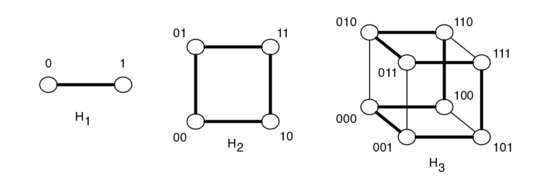
\includegraphics[scale=0.8]{images/hipercubo.png} 
\end{center}

\item Três marinheiros naufragaram em uma ilha e eles coletaram uma grande pilha de cocos durante o dia. Naquela noite, o primeiro marinheiro acorda e decide pegar sua primeira porção mais cedo, então tenta dividir a pilha de cocos igualmente em três pilhas, mas descobre que sobrou um coco, então ele o joga para um macaco e depois esconde sua parte das três pilhas de cocos do mesmo tamanho e junta as outras duas pilhas juntas para formar uma única pilha visível de cocos novamente e vai para a cama.

Para encurtar a história, cada um dos marinheiros, por sua vez, se levanta uma vez durante a noite e executa as mesmas ações de dividir a pilha de coco em três, descobrindo que sobrou um coco e dando aquele único coco restante ao macaco.

Pela manhã (após a ação clandestina e separada de cada um dos cinco marinheiros durante a noite), os cocos restantes são divididos em três pilhas iguais para cada um dos marinheiros, após o que se verifica que a pilha de cocos se divide igualmente entre os marinheiros sem resto. (Nada para o macaco pela manhã.)

Faça um programa que dado um inteiro N representando o número inicial de marinheiros encontre o número piha de cocos coletadas inicialmente. 

\textbf{Entrada}

Uma linha contendo um inteiro (N  $\leq$ 9 ) representando o número de marinheiro.

\textbf{Saída}

Devolva um inteiro representando o número de coco coletados inicialmente.\\

\textbf{Entrada}\\
3\\

\textbf{Saída} \\
25\\

\item \textbf{TapiocaSort} Preparar a pilha perfeita de tapiocas é uma tarefa complicada, porque não importa como você tenta todas as tapiocas em qualquer pilha têm diâmetros diferentes. Para o bem da limpeza, no entanto, você pode ordenar a pilha por tamanho de forma que cada tapioca seja menor do que todos os panquecas abaixo dela. O tamanho de uma panqueca é dado pelo seu diâmetro.

A ordenação de uma pilha é feita por uma sequência de "viradas" de tapiocas. Uma virada consiste em inserir uma espátula entre duas tapiocas em uma pilha e virando (invertendo) todas as panquecas em a espátula (invertendo a subpilha).

Uma virada é especificado dando a posição da tapioca na parte inferior da subpilha a ser virada em relação a toda a pilha. A panqueca de baixo tem a posição 1, enquanto a panqueca de cima em uma pilha de n panquecas tem posição n.

Uma pilha é especificada dando o diâmetro de cada tapioca na pilha na ordem em que aparecem as tapiocas. Por exemplo, considere uma pilha de tapiocas abaixo em que a tapioca 5 é a primeira tapioca do vetor:

topo -> 5 1 2 3 4 |

Fazendo a operação virada 1 (a espátula está representada por |), obtemos a seguinte pilha de tapiocas:

topo -> 4 3 2 1 | 5

Fazendo a operação virada 2, obtemos a seguinte pilha de tapiocas:

topo -> 1 2 3 4 5

Observe que a pilha de tapioca pode ser ordenada utilizando duas operações de virada.

\textbf{Entrada}

A primeira linha da entrada contém um inteiro N representando o número de tapiocas.

A segunda linha contém N inteiros positivos representando uma pilha de tapiocas. Cada tapioca terá um diâmetro entre 1 e 30.

\textbf{Saída}

Seu programa deve imprimir uma sequência de viradas que resulte na pilha de tapioca ordenada de maneira que a maior tapioca está na parte inferior e a menor tapioca na parte superior. A sequência de viradas deve terminar com 0, indicando que não são mais necessárias viradas.


\begin{tabular}{|l|l|}
\hline
Exemplo de Entrada & Exemplo de Saída\\
5                & 1 2 0\\      
5 1 2 3 4        &\\
\hline
\end{tabular}


\begin{tabular}{|l|l|}
\hline
Exemplo de Entrada & Exemplo de Saída\\
5                & 1 0\\      
5 4 3 2 1        &\\
\hline
\end{tabular}

\item  Pão a metro é um tipo de sanduíche gigante que é uma excelente opção de lanche para torneios de programação, embora a experiência já tenha mostrado que o oferecimento de sanduiches pode gerar reclamação dos competidores. Outro grande problema é que algumas pessoas são mais gulosas que outras e, dessa maneira, acabam pegando pedaços maiores que os pedaços dos outros. Para a final da OBI, a coordenação estava pensando em providenciar pão a metro para os competidores, porém tais problemas os fizeram recuar na idéia.

Embora a idéia tenha sido momentaneamente abandonada, uma idéia simples surgiu: cortar previamente o pão em fatias de tamanho iguais e distribuí-las entre as pessoas. O único problema com tal idéia é que se o número de pessoas for muito grande, fica impraticável ter apenas um pão. Por exemplo, se quisermos que 1.000 pessoas recebam 20 centímetros de sanduíche, seria necessário um sanduíche de 20.000 centímetros, ou 200 metros!

Alguém levantou a seguinte hipótese: se houvesse N pessoas e fossem encomendados K sanduíches de empresas diferentes, cada qual com uma determinada metragem (tamanho) $M_i$ ($1 \leq i \leq K$), seria possível retirar desses pães N fatias de mesmo tamanho, possivelmente sobrando partes nao utilizadas. A questão seria: qual o tamanho inteiro máximo que essas fatias poderão ter?

Por exemplo, se tivermos K = 4, com os tamanhos (em centímetros) M1 = 120, M2 = 89, M3 = 230 e M4 = 177 e N = 10, podemos retirar N fatias iguais de tamanho máximo 57, pois assim conseguimos 2 fatias no primeiro pão, 1 no segundo, 4 no terceiro e 3 no quarto, totalizando as 10 fatias necessárias. Se tentarmos cortar fatias de tamanho 58, só será possível obter 3 fatias do terceiro pão, totalizando 9 e, portanto, 57 é realmente o melhor que podemos obter. Note que não podemos usar duas ou mais fatias menores de diferentes pães para formarmos uma fatia do tamanho selecionado. (ficaria muito deselegante dar um lanche recortado às pessoas).

Tarefa

Escreva um programa que, dados os tamanhos de pão disponíveis (em centímetros) e a quantidade de pessoas a serem atendidas, retorne o tamanho inteiro máximo (em cent ímetros) da fatia que pode ser cortada de maneira a atender todas as pessoas.

Entrada

A entrada contém um único conjunto de testes, que deve ser lido do dispositivo de entrada padrão (normalmente o teclado). A primeira linha da entrada contém um inteiro N que indica a quantidade pessoas ($1 \leq N \leq 10.000$). A segunda linha contém um inteiro K ($1 \leq K \leq 10.000$) que é a quantidade de sanduíches disponível. Na terceira linha há K inteiros M ($1 \leq M \leq 10.000$) separados por um espaço em branco representando o tamanho de cada pão.

Saída Seu programa deve imprimir, na saída padrão, uma única linha, contendo o tamanho inteiro máximo da fatia que pode ser cortada.

Exemplos


\begin{tabular}{|l|l|}
\hline
Entrada & Saída\\
\hline
10                & 57\\      
4        &\\
120 89 230 77 & \\
\hline
\end{tabular}


    
\end{enumerate}




















\section{Backtracking}

O algoritmo de backtracking pode ser entendido como um refinamento de um algoritmo de força bruta. No algoritmo de backtracking, a solução para um problema computacional é construída de maneira incremental assim que uma condição do problema é violada, o algoritmo retrocede e tenta a próxima alternativa.

Vamos exemplificar o funcionamento de um algoritmo de backtracking na solução de um problema de satisfação. Um problema de satisfação pode ser definido por uma tripla $(X, D, C)$ onde:

\begin{itemize}
    \item $X = \{X_1, X_2, \ldots, X_n\}$ é um conjunto de variáveis.
    \item $D = \{D_1, D_2, \ldots, D_n\}$ é o conjunto dos respectivos domínios de cada variável.
    \item $C = \{C_1,C_2, \ldots,C_m\}$ é o conjunto de restrições do problema.
\end{itemize}


\begin{algorithm}
  \caption{Algoritmo de Backtracking}\label{AIPal}
  \begin{algorithmic}
    \Function{Backtracking}{$i,n$}
    
    \If{i = n+1}
        \State save\_solution(X)
    \Else 
        \For{$j \in D_i$}
            \If{$X[i] = j$ não viola nenhuma restrição}
            \State X[i] $\leftarrow$ j
            \State Backtracking(i+1, n)
            \EndIf
        \EndFor
    \EndIf
     
    \EndFunction
  \end{algorithmic}
\end{algorithm}

\subsection{Problema das n rainhas}

No problema das $n$ rainhas, temos n variáveis $(Q[1],Q[2], \ldots, Q[n])$. Cada variável $Q[i]$ guarda a posição da linha da i-ésima rainha. Em tabuleiro $n \times n$, $Q[i] \in \{1, 2, \ldots, n\}$. Neste problema, temos $n$ variáveis e seus domínios tem $n$ valores distintos.  As restrições para o problema são as seguintes:

\begin{enumerate}
    \item $\forall { 1 \leq  i < j \leq n} \quad Q[i] \neq Q[j] $
    \item $\forall { 1 \leq  i < j \leq n} \quad Q[i] + i \neq Q[j] + j$.
    \item $\forall { 1 \leq  i < j \leq n} \quad Q[i] - i \neq Q[j] - j$.
\end{enumerate}

A restrição (1) garante que não teremos duas rainhas distintas na mesma linha. A restrição (2) garante que não teremos duas rainhas na mesma diagonal secundária. A restrição (3) garante que não teremos duas rainhas na mesma diagonal principal. 

No algoritmo de backtracking, essas restrições são verificadas de maneira incremental considerando as fixações das variáveis já realizadas.

O Código abaixo escrito em C++ implementa o algoritmo de backtracking para o problema da n rainhas descrito acima.

\begin{minted}{C++}
void place_queen(vector <int> Q, int r, int n, int & cont){
    if(r == n+1){
        cont++;
    }else{
        for(int j = 1; j <= n; j++){
            bool legal = true;
            for(int i = 1; i <= r-1; i++){
                if( Q[i] == j || Q[i] == j+r-i || Q[i] == j-r+i){
                    legal = false;
                }
            }
            if(legal){
                Q[r] = j;
                place_queen(Q, r+1, n, cont);
            }
        }
    }
}

\end{minted}

\subsection{Problema da soma de subconjuntos}

Dado um conjunto $S$ com $n$ elementos encontre um subconjunto $S' \subseteq S$ tal que a soma dos elementos de $S'$ seja igual a um valor $K$.

Esse problema pode ser modelado da seguinte maneira. Teremos $n$ variáveis $(X[1], X[2], \ldots, X[n])$. Cada variável X[i] pode assumir dois valores \{true, false\}. Se X[i] é true, então $S[i] \in S'$. Caso contrário $S[i] \not \in S'$.

O nosso problema terá uma única restrição:

\begin{itemize}
    \item $\sum_{i=1}^{n} X[i]\cdot S[i] = K$
\end{itemize}

O Código abaixo escrito em C++ implementa o algoritmo de backtracking para o problema da soma de subconjunto.

\newpage 

\begin{minted}{C++}
void subsetsum(vector <int> & S,vector <bool> X, int K, int i, int n){
    if(i == n){
        bool flag = true;
        cout << "{";
        for(int j = 0; j < i; j++){
            if(X[j])
                cout << S[j] << " ";
        }
        cout << "}" << endl;
    }else{
        int prev = 0;
        for(int j = 0; j < i; j++){
            if(X[j])
                prev += S[j];
        }
        
        int next = 0;
        for(int j = i+1; j < n; j++){
            next += S[j];
        }

        
        if(prev + next >= K){            
            X[i] = false;
            subsetsum(S, X, K,  i+1, n);
        }
        
        if(prev + S[i] <=  K){
            X[i] = true;
            subsetsum(S, X, K, i+1, n);
        }
    }
}

int main(){
    
    vector <int> S( {2,3,4,1,7,8});
    vector <bool> X;
    X.resize(S.size());
    int K = 5;
    subsetsum(S, X, K, 0, S.size());
}

//Output:
//{4 1 }
//{2 3 }

\end{minted}

\subsection{Exercícios}

\begin{enumerate}
\item 

No quebra-cabeças Unruly, você recebe um tabuleiro $n \times n$. Cada quadrado do tabuleiro é colorido inicialmente com as cores branco, preto e cinza. O objetivo do jogo é pintar cada quadrado com a cor cinza com preto ou branco, de forma que:

\begin{itemize}
    \item não há três quadrados consecutivos, horizontalmente ou verticalmente, são da mesma cor
    \item cada linha e coluna contém o mesmo número de quadrados pretos e brancos. 
\end{itemize}

\begin{center}
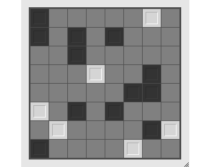
\includegraphics[scale=0.8]{images/unruly.png} 
\end{center}

Desenvolva um algoritmo de backtracking que resolva esse quebra-cabeça.

O jogo pode ser encontrado no seguinte link: \url{https://www.chiark.greenend.org.uk/~sgtatham/puzzles/js/unruly.html}

\item No quebra-cabeças Rectangles, você recebe uma grade retangular e alguns quadrados numerados.

\begin{center}
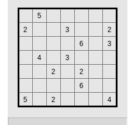
\includegraphics[scale=1.0]{images/Rectangles.png} 
\end{center}

Seu objetivo é traçar linhas paralelas as bordas grade rectangular para dividir a grade em retângulos, de modo que cada retângulo contenha exatamente um quadrado numerado e sua área seja igual ao número escrito naquele quadrado.

\begin{center}
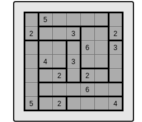
\includegraphics[scale=1.0]{images/Rectangles2.png} 
\end{center}

O jogo pode ser encontrado no seguinte link: \url{https://www.chiark.greenend.org.uk/~sgtatham/puzzles/js/rect.html}


\end{enumerate}






%\subsection{Maior subsequência crescente (Longest Increasing Subsequence)}

%Dado um vetor inteiro $A[1..n-1]$, nós precisamos encontrar a maior sequência de índices $i_1,i_2, \ldots, %i_l$ tal que $1 \leq i_1 < i_2 < \ldots < i_l \leq n$ e $A[i_1] < A[i_2] < \ldots < A[i_l]n$ 




% \section{Definição recursivas de conjuntos}

% Alguns conjuntos podem ser definidos de maneira recursiva. O conjuntos dos números pares positivos $P$ pode ser definido recursivamente da seguinte maneira:

% \begin{itemize}
%     \item $0 \in P$
%     \item Se $n \in P$ eentão $n+2 \in P$.
% \end{itemize}


% %Considere uma definição alternativa do conjuntos dos números pares positivos de maneira explicíta: 
% %\begin{equation}
% %P' = \{ 2k | k \in \mathbb{N} \}    
% %\end{equation}

% %É fácil mostrar que $P = P'$. 

% Seja S o conjunto dos pares ordenados de inteiros positivos $(a,b)$ tal que $2 | a + b$ pode ser definido recursivamente da seguinte maneira:

% \begin{itemize}
%     \item Passo Base: $(0,0) \in S$
%     \item Passo Recursivo Se $(a,b) \in S$ então $(a+1,b+1),(a+2,b),(a,b+2) \in S$.
% \end{itemize}

% O conjunto de todos os subconjuntos de um conjunto A, $subsets(A)$, pode ser definido recursivamente da seguinte maneira:

% \begin{itemize}
%     \item Passo Base: $\emptyset \in subsets(A)$
%     \item Passo Recursivo Seja $x \in A$, $Y \in subset(A\setminus \{x\})$ então $Y, Y \cup \{x\} \in subsets(A)$.
% \end{itemize}











